\begin{frame}{$\chi_{b1,2}(1,2,3P) \to \OneS \gamma$ fit model}
\begin{columns}
\column{.5\textwidth}
  \centering
  \setlength{\unitlength}{1mm}
  \begin{picture}(50,80)
      %
    \put(0,0){
      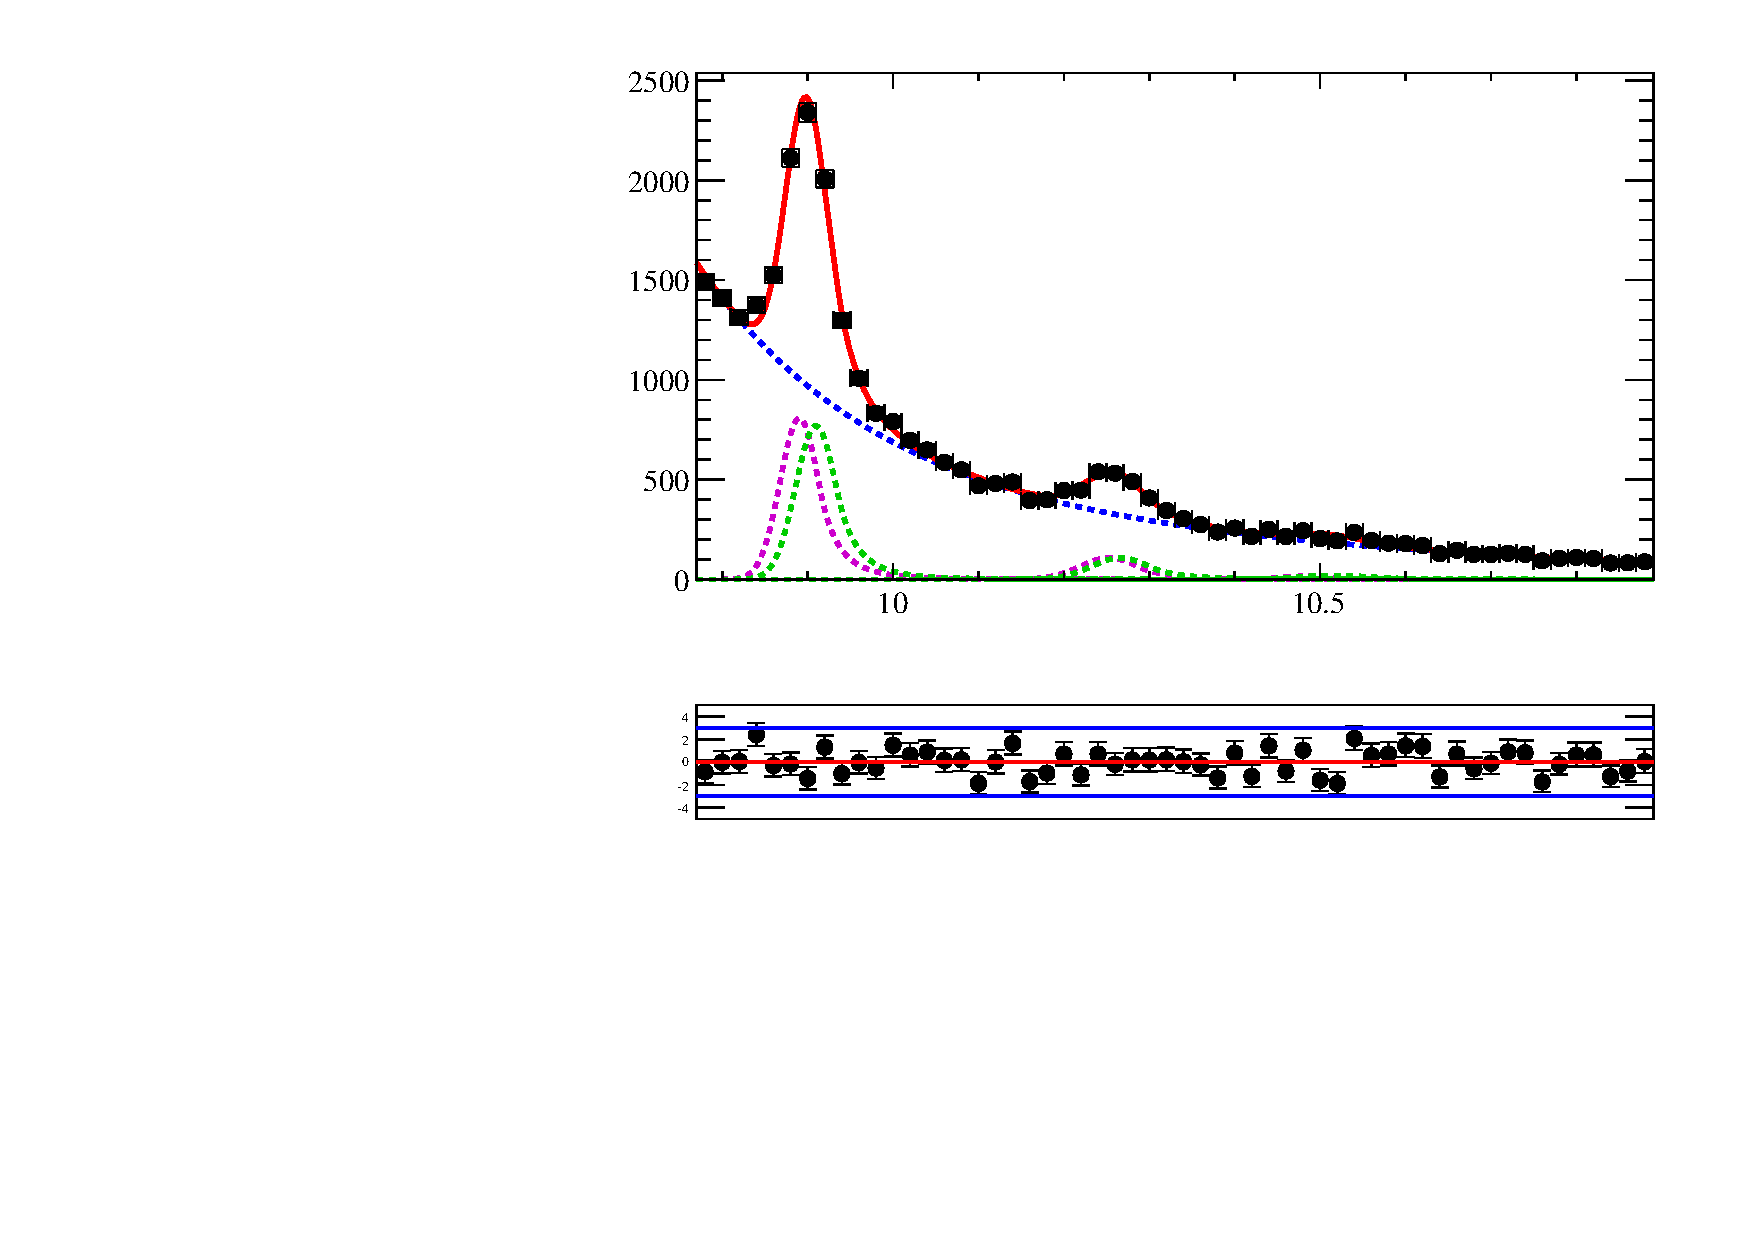
\includegraphics[width=50mm, height=40mm]{chib1s-fit/f2012_14_40}
    }
    
    \put(0,40){
      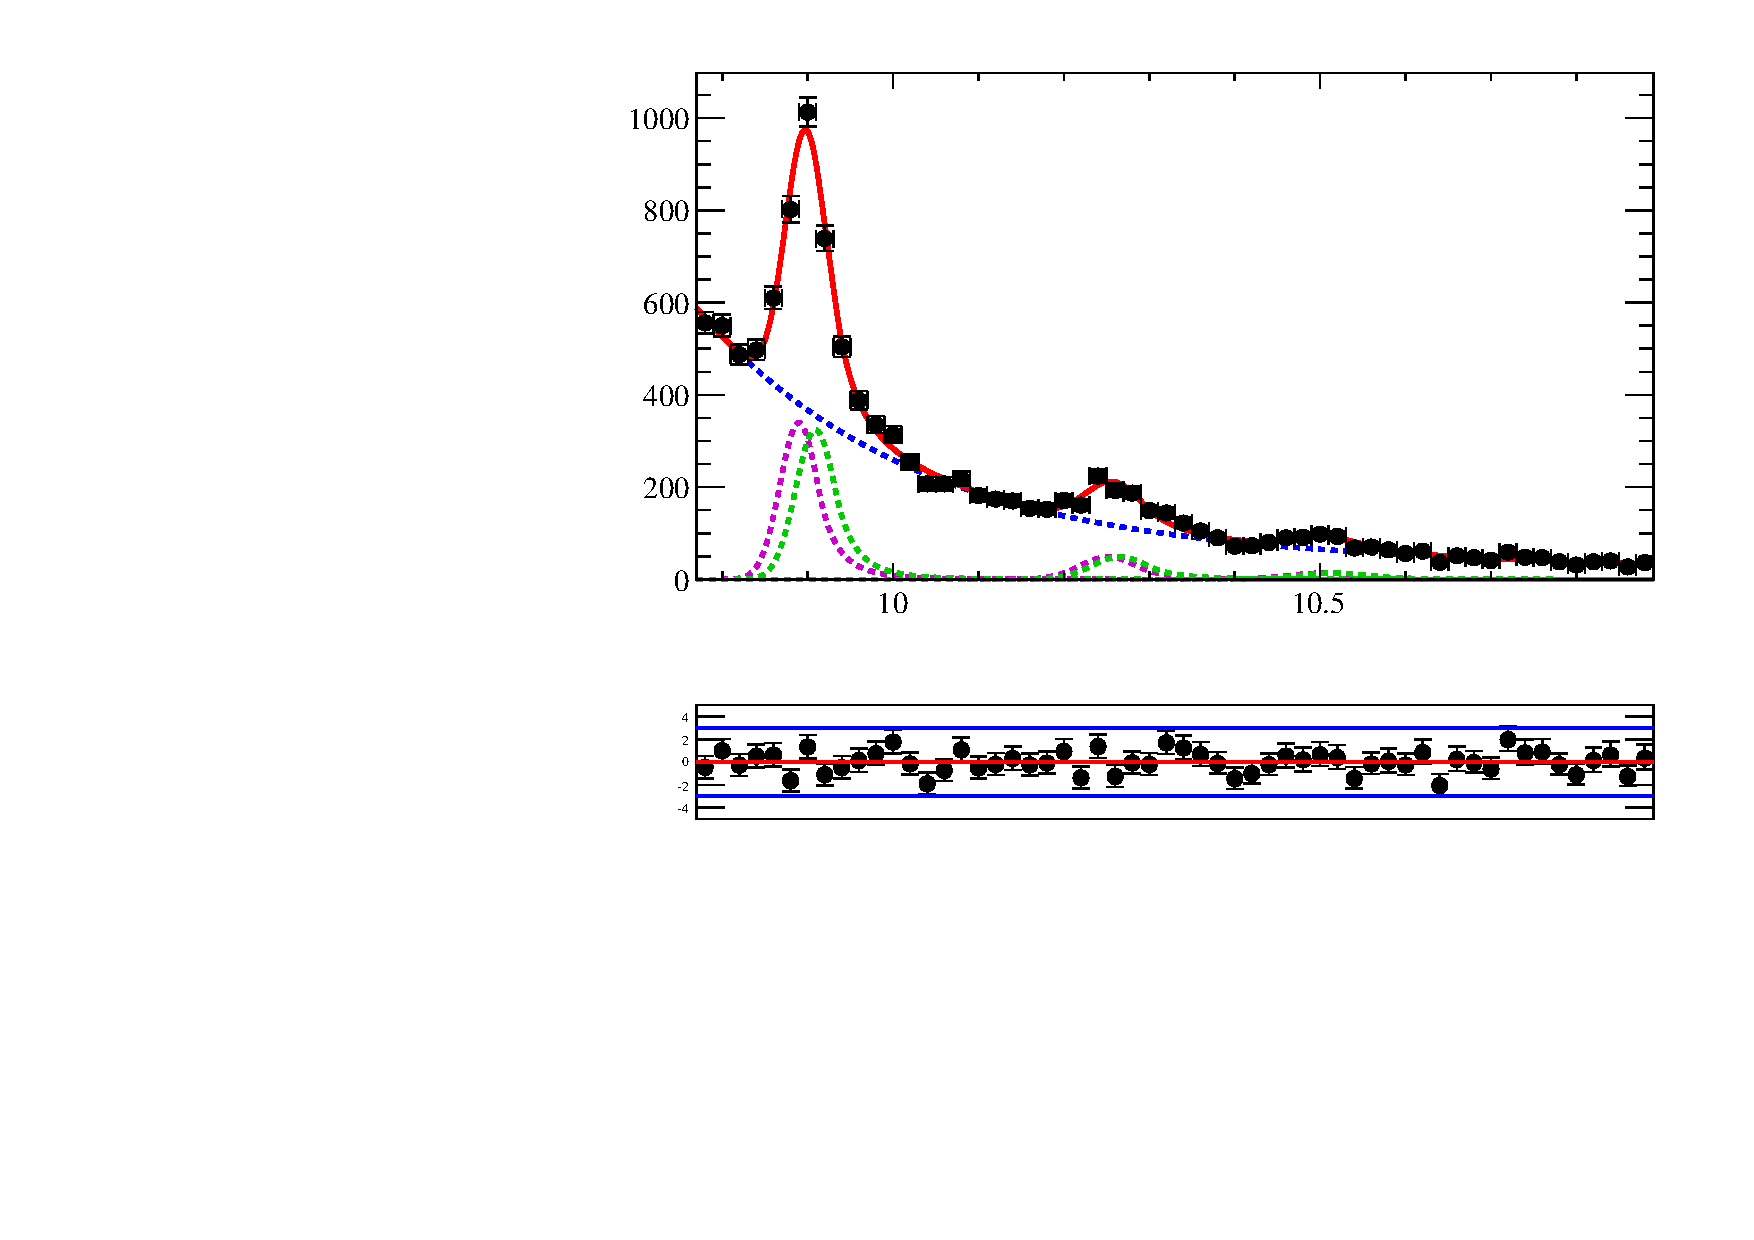
\includegraphics[width=50mm, height=40mm]{chib1s-fit/f2011_14_40}
    }

    \put(0,15){\tiny \begin{sideways}Candidates/(20\mevcc)\end{sideways}}
    \put(5,9){\tiny $m_{\mumu \gamma} - m_{\mumu} + m_{\Y1S}^{PDG} \left[\gevcc\right]$}
    \put(25,30){$\sqrt{s} = 8\tev$}
    \put(16,25){\tiny $14 < p_T^{\Y1S} < 40 \gevc$}
    
    \put(0,55){\tiny \begin{sideways}Candidates/(20\mevcc)\end{sideways}}
    \put(5, 49){\tiny $m_{\mumu \gamma} - m_{\mumu} + m_{\Y1S}^{PDG} \left[\gevcc\right]$}
    \put(25,70){$\sqrt{s} = 7\tev$}
    \put(16,65){\tiny $14 < p_T^{\Y1S} < 40 \gevc$}
    
    \put(15,75){\tiny \chibOneP}
    \put(25,60){\tiny \chibTwoP}
    \put(35,57){\tiny \chibThreeP}
    \put(15,35){\tiny \chibOneP}
    \put(25,20){\tiny \chibTwoP}
    \put(35,17){\tiny \chibThreeP}
        

    % \graphpaper[5](0,0)(50, 80)        
  \end{picture}
\column{.5\textwidth}
\begin{itemize}
\item One Crystal Ball (CB) for each $\chi_{b1,2}(1P,2P,3P)$ state: 6 CB in total
\item Exclude the study of $\chi_{b0}$ due to its low radiative branching ratio.
\item Product of exponential and linear combination of 
polynomials  for combinatorial background.
\end{itemize}
\end{columns}
\end{frame}
